\section{网络实现细节 (Implementation Details of the Network)}
\subsection{感知与预测架构 (Architecture for Perception and Prediction)}

\subsubsection{时空感知 (Spatial-Temporal Perception).}
% \textbf{Spatial Fusion.}
针对 nuScenes 数据集，首先将原始图像 $\mathbb{R}^{3 \times 900 \times 1600}$ 裁剪并缩放到 $\mathbb{R}^{3 \times 224 \times 480}$，取过去 3 帧输入模型，记作 $I_t^n \in \mathbb{R}^{3 \times 224 \times 480}$，其中 $t \in \{1,2,3\}, n \in \{1,\dots,6\}$。
%
采用 EfficientNet-B4~\cite{tan2019efficientnet} 作为主干网络 (backbone)，获得特征 $f_i^k \in \mathbb{R}^{C \times H_e \times W_e}$ 和深度估计 (depth estimation) $d_i^k \in \mathbb{R}^{D \times H_e \times W_e}$，其中 $C = 64, D = 48, H_e = 28, W_e = 60$。
%
深度范围 $2m$ 到 $50m$，间隔 $1m$。
%
将特征沿整条光线空间按预测深度分布展开后，所有视角的相机图像记为 $u_i^k \in \mathbb{R}^{C \times D \times H_e \times W_e}$。
%
然后利用自车运动 (ego-motion) 矩阵，将所有环视相机及时间戳的特征变换到以 $t$ 时刻自动驾驶车辆 (SDV, Self-driving vehicle) 为中心的坐标系，得到自我中心 (ego-centric) 特征 $\{u_i^{'}\}$。
%
最后，鸟瞰图 (BEV) 特征图 $b_i \in \mathbb{R}^{C \times H_b \times W_b}$ 可从 $\{u_i^{'}\}$ 经求和池化得到，其中 $H_b =200, W_b = 200$。

% \noindent
% \textbf{Temporal Fusion.} 
为增强特征，可通过时序融合 (temporal fusion) 步骤中的累积方法将历史信息集成到每一帧。
%
然后将这些特征送入由 3D 卷积实现的时序模型 (temporal model)，以更好对齐时序特征。
%
具体而言，为涵盖不同感受野，在时间通道上采用不同 3D 卷积核大小 $[(2,3,3),(1,3,3)]$，以及核大小为 $(2,200,200)$ 的金字塔池化。
%
将所有输出拼接后送入最终压缩卷积层，得到最终输出 $x_{1 \sim t} \in \mathbb{R}^{C \times H_b \times W_b}$。
%
输出特征经过时序模型后保持与输入相同形状，来自不同时间戳的特征得以集成。

\noindent
\subsubsection{未来预测 (Future Prediction).}
实验中通过两种不同分布建模未来不确定性 (uncertainty distribution)：高斯分布 (Gaussian distribution) 和 Bernoulli分布 (Bernoulli distribution)。
%
对于高斯分布，当前特征 $x_t$ 经过若干残差块 (residual block) 层和平均池化 (average pooling) 层，得到隐状态 (hidden state) $\mathbb{R}^{32 \times 1 \times 1}$。
%
然后使用核大小为 $(1,1)$ 的 2D 卷积拟合高斯分布的均值和 log 方差，尺寸为 $R^{32} \times R^{32}$。
%
对于 Bernoulli分布，由于每个空间网格为 $0-1$ 值，将 $x_t$ 送入若干残差块层后经 LogSigmoid 回归每个网格的概率。
%
预测网络利用卷积 GRU（门控循环单元, Gated Recurrent Unit）作为基本模块，每个门由步长为 $3$ 的 2D 卷积实现。
%
通过一个具有 2 个输出通道的信任门（由 2D 卷积实现）合并预测特征，并将该门作为权重对两个预测特征求和。
%
合并后的预测特征作为"不确定性"路径的隐状态和"历史"路径的输入状态。
%
通过此方法，可递归预测未来状态 $(\hat{x}_{t+1},\dots, \hat{x}_{t+H})$。

\noindent
\subsubsection{BEV表示解码器 (Decoders for BEV Representations).}
考虑解码器 (decoder) 鲁棒性，所有任务头共享同一主干网络，该主干网络由 ResNet-18~\cite{he2016resnet} 前三层和三个上采样因子为 2 的含跳跃连接的上采样层实现。
%
特征现为 64 通道，随后按任务需求送入不同头部。每个头部由两个具有不同输出通道的 2D 卷积组成。
%
具体而言，语义分割 (semantic segmentation) 头输出通道数均设为 2。而实例分割 (instance segmentation) 任务需预测偏移量、中心、未来光流，因此分别设为 2、1 和 2。





\subsection{规划 (Planning)}
本节详细说明评分函数和优化 GRU 网络 (refinement GRU network) 的实现。

\noindent\textbf{安全代价 (Safety Cost).} 自动驾驶车辆 (SDV) 不应与道路上其他物体碰撞，规划轨迹 (trajectory) 时需考虑其未来运动。
%
为此，利用预测占用图 (occupancy map) 对与占用区域相交的轨迹施加惩罚。
%
形式化地，对每个时间戳 $t$ 的轨迹 $\tau$，若 SDV 多边形 $g$ 与其它物体占用网格相交（含安全裕度参数 $\lambda$），则对 $\tau$ 施加惩罚，记作 $o_g(\tau, t, \lambda)$。与物体碰撞相关的安全代价 (safety cost) 如下：
\begin{equation}
    f_o(\tau, o) = \sum_t \sum_g o_g(\tau, t, 0) + o_g(\tau, t, \lambda) v(\tau, t),
\end{equation}
其中第一项惩罚相交网格，第二项以不确定性占用惩罚高速运动。

此外，SDV 通常跟随前车并保持一定安全距离，这主要取决于前车速度。
%
由于高清地图 (HD map) 不可用且无法获取沿中心车道的前车信息，转而根据 SDV 速度确定距离 $L$，计算 SDV 前方占用网格。
%
因此，若与前车距离过近，代价将增大，该轨迹将被判定为不佳。
%
但在变道操作中此方法无效，因为前车并非正对 SDV 前方。

上述目标关注运动物体，同时车辆也应保持在车道线中央。
%
可通过第一阶段感知的车道来保障行车安全，代价函数设为距车道线的距离。


\noindent\textbf{优化 (Refinement).} 根据评分函数选出轨迹 $\tau^*$ 后，通过 GRU 网络进行优化。具体而言，GRU 的隐状态为编码器前视相机特征，输入状态为当前位置、所选轨迹 $\tau^*$ 位置和目标点的拼接。注意初始当前位置为 $(0,0)$。通过相同过程，可递归获得最终优化轨迹，该轨迹考虑了前视相机信息和目标点信息。








\section{深度监督 (Depth Supervision)}

本节介绍如何生成 nuScenes 数据集深度图用于显式监督。

采用名为 FSRE-Depth~\cite{Jung_2021_ICCV} 的带语义分割的自监督方法，该方法在深度生成方面表现优异。由于 FSRE-Depth 以语义分割作为输入，先在 Mapillary Vistas Dataset~\cite{Mapillary} 上训练分割模型，然后应用于 nuScenes 数据集生成语义结果，如图 \ref{fig:depth_vis}(b) 所示。
%
下一步，以 ResNet-50 为主干网络，使用 nuScenes 前视图像训练 FSRE-Depth。输入图像分辨率为 $1216 \times 672$。经过 45 个 epoch 训练后，模型可预测前视图像的充分结果。为充分发挥深度模型性能，进一步在每个相机视角上训练 15 个 epoch。
%
由此，该模型可分别生成所有相机视角的深度图。为评估深度图质量，每间隔 20 帧使用 LiDAR 点计算深度估计指标。结果如表 \ref{tab:depth_map_eval} 所示，表明深度图质量良好。
%
图 \ref{fig:depth_vis}(c) 所示结果将用于显式监督 ST-P3 感知模块中的深度估计 (depth estimation)。


% \begin{figure}[tb!]
%     \centering
%     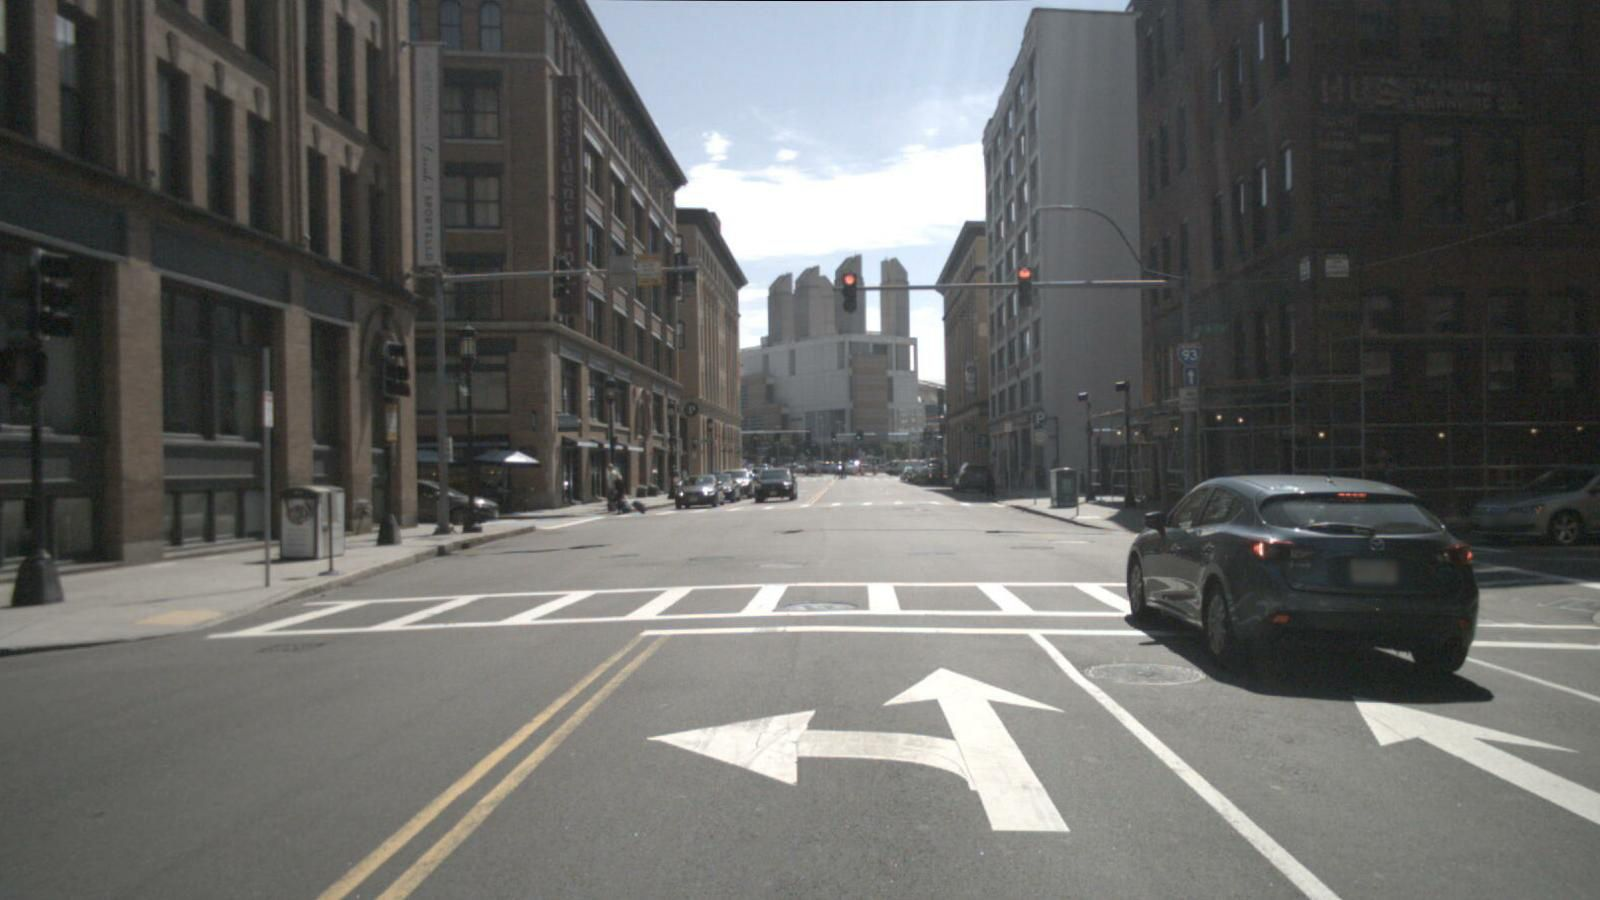
\includegraphics[width=0.8\textwidth]{Figs/depth_origin.jpg}
%     \caption{Original image in nuScenes dataset for depth generation}
%     \label{fig:depth_origin}
% \end{figure}
% \begin{figure}[tb!]
%     \centering
%     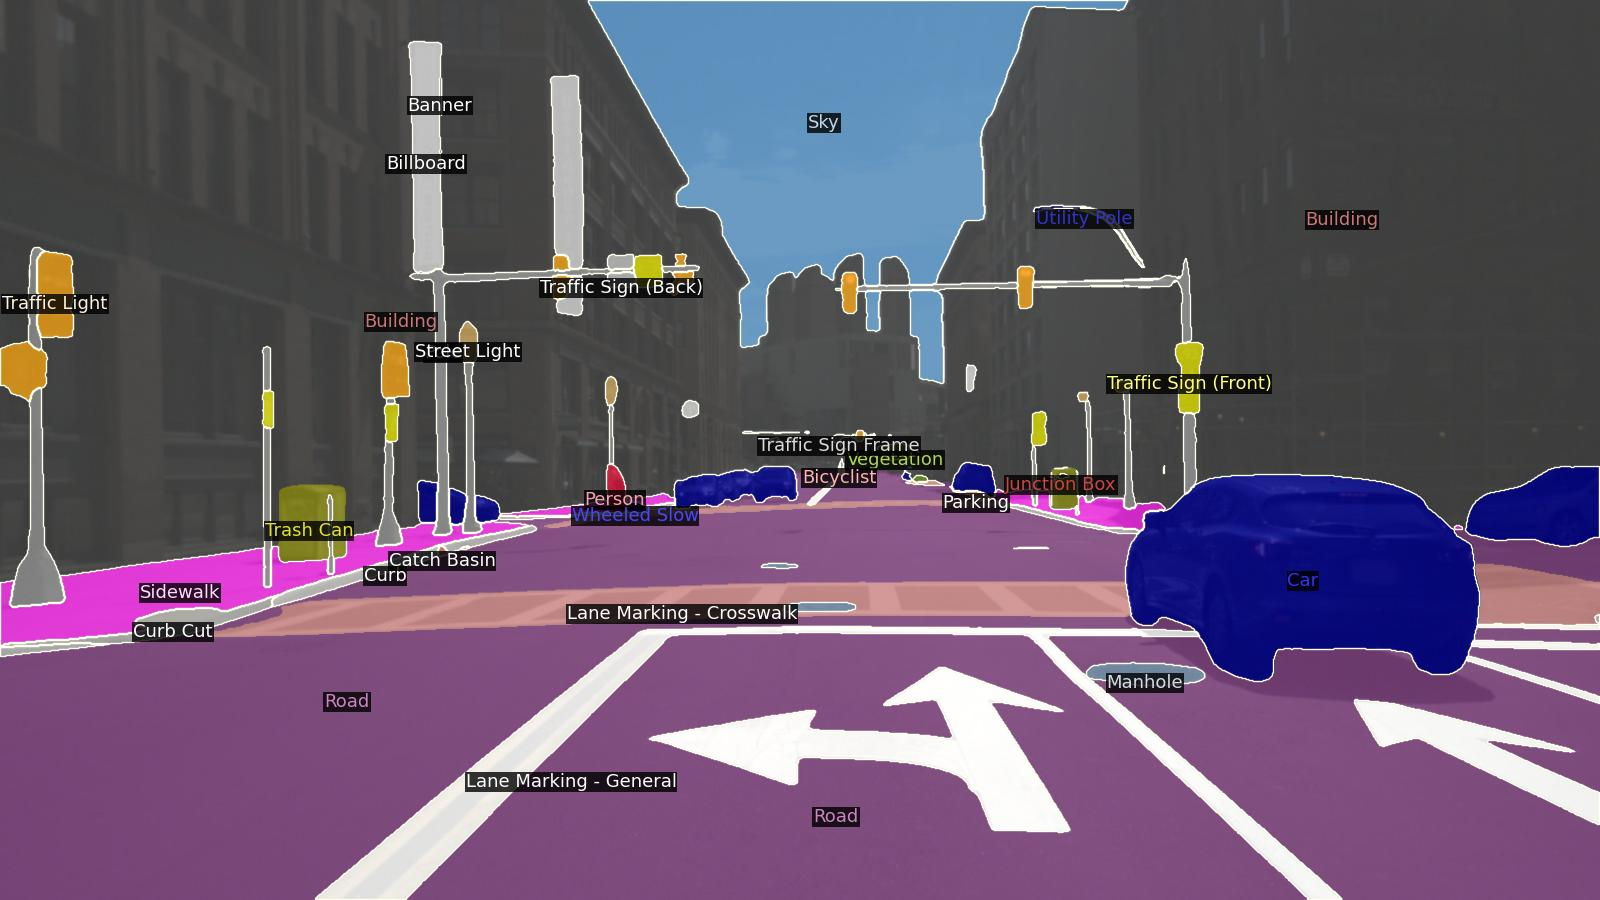
\includegraphics[width=0.8\textwidth]{Figs/depth_seg.jpg}
%     \caption{Segmentation result}
%     \label{fig:depth_seg}
% \end{figure}
% \begin{figure}[tb!]
%     \centering
%     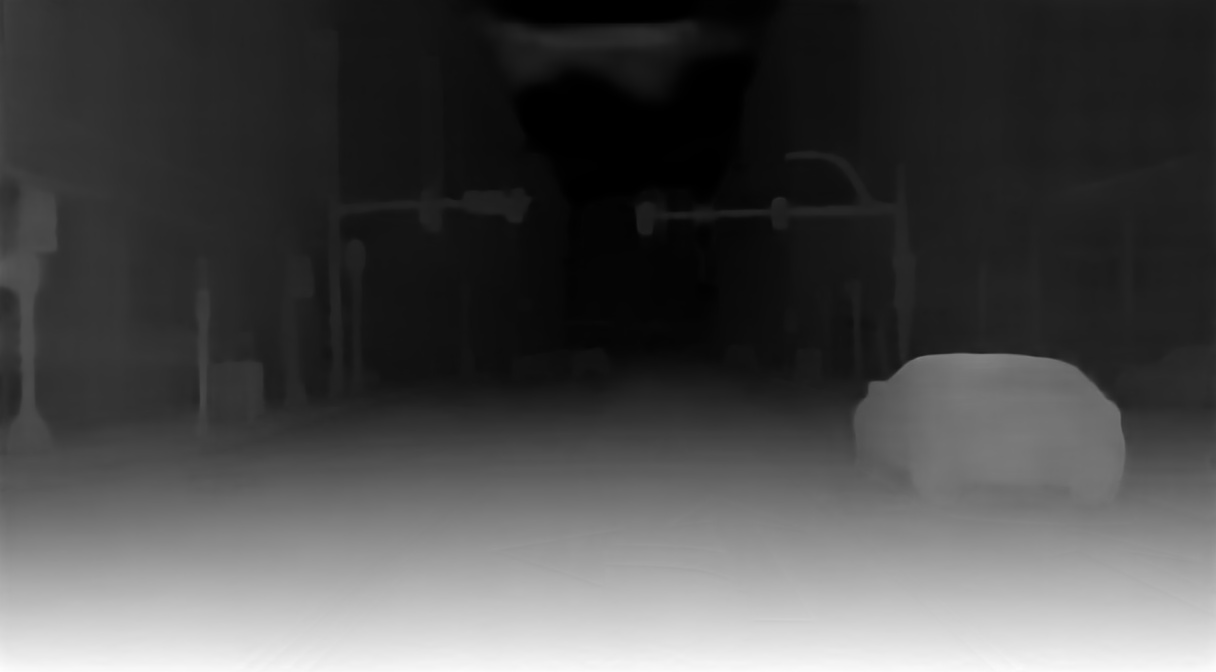
\includegraphics[width=0.8\textwidth]{Figs/depth_depth.jpg}
%     \caption{Predicted depth map}
%     \label{fig:depth_depn}
% \end{figure}


\begin{figure}[tb!]
    \centering
    \subfigure[]{
    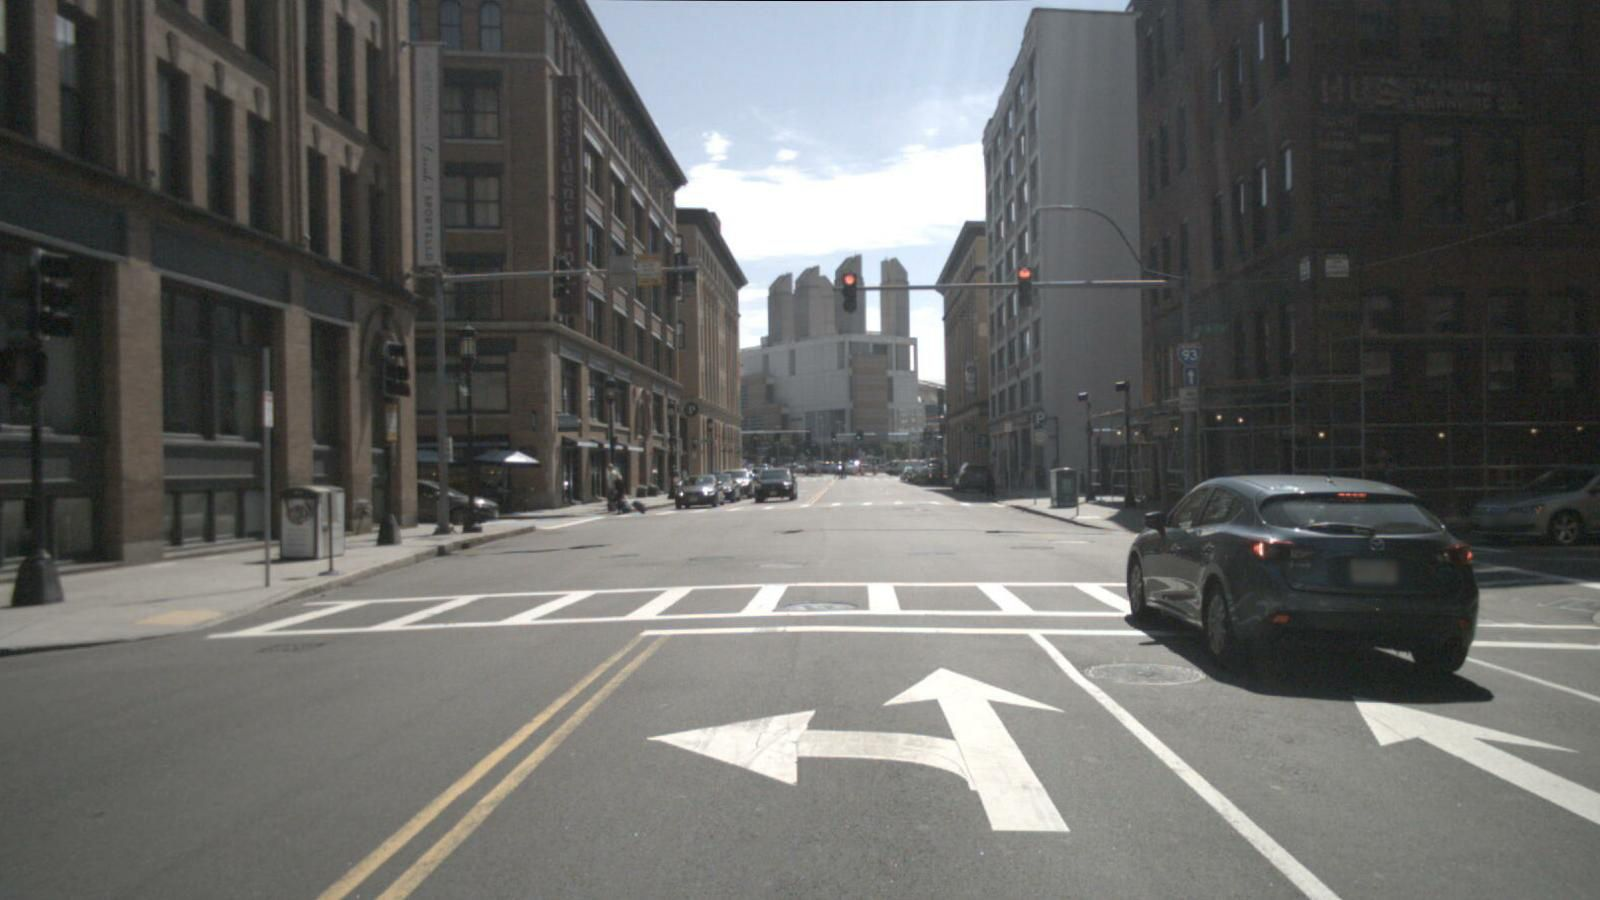
\includegraphics[width=0.75\textwidth]{Figs/depth_origin.jpg}
    }
    \quad
    \subfigure[]{
    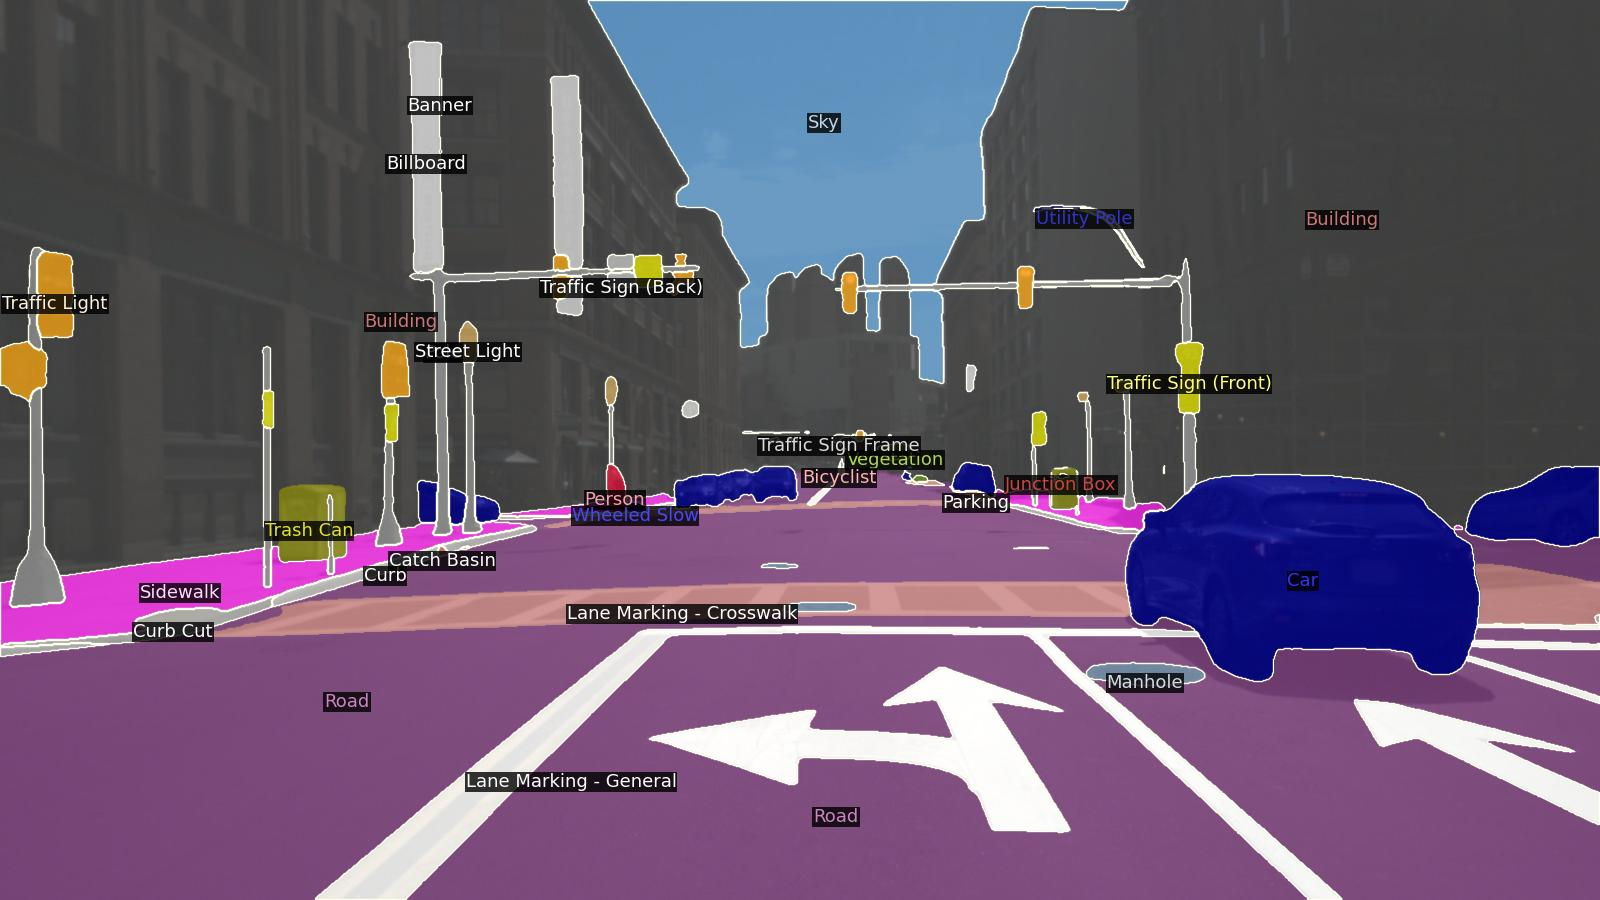
\includegraphics[width=0.75\textwidth]{Figs/depth_seg.jpg}
    }
    \quad
    \subfigure[]{
    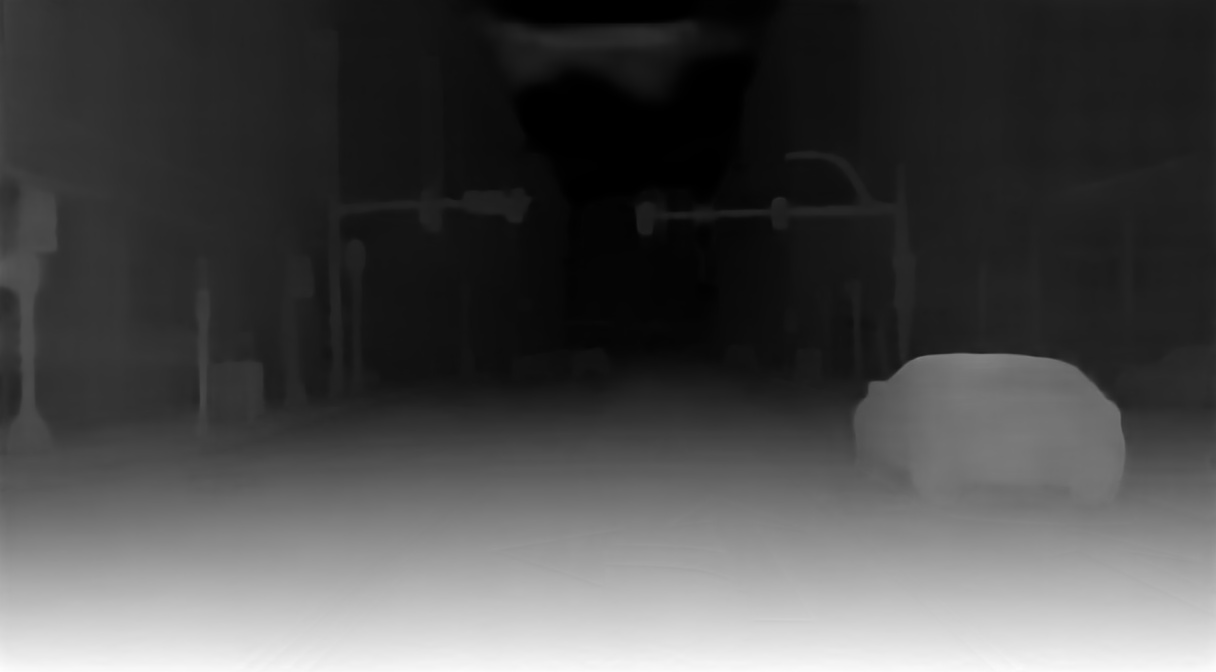
\includegraphics[width=0.75\textwidth]{Figs/depth_depth.jpg}
    }
    \caption{(a) 原始图像 (Original image); (b) 分割结果 (Segmentation result); (c) 预测深度图 (Predicted depth map)}
    \label{fig:depth_vis}
\end{figure}


% \begin{figure}[tb!]
%     \centering
%          \begin{subfigure}[b]{0.3\textwidth}
%              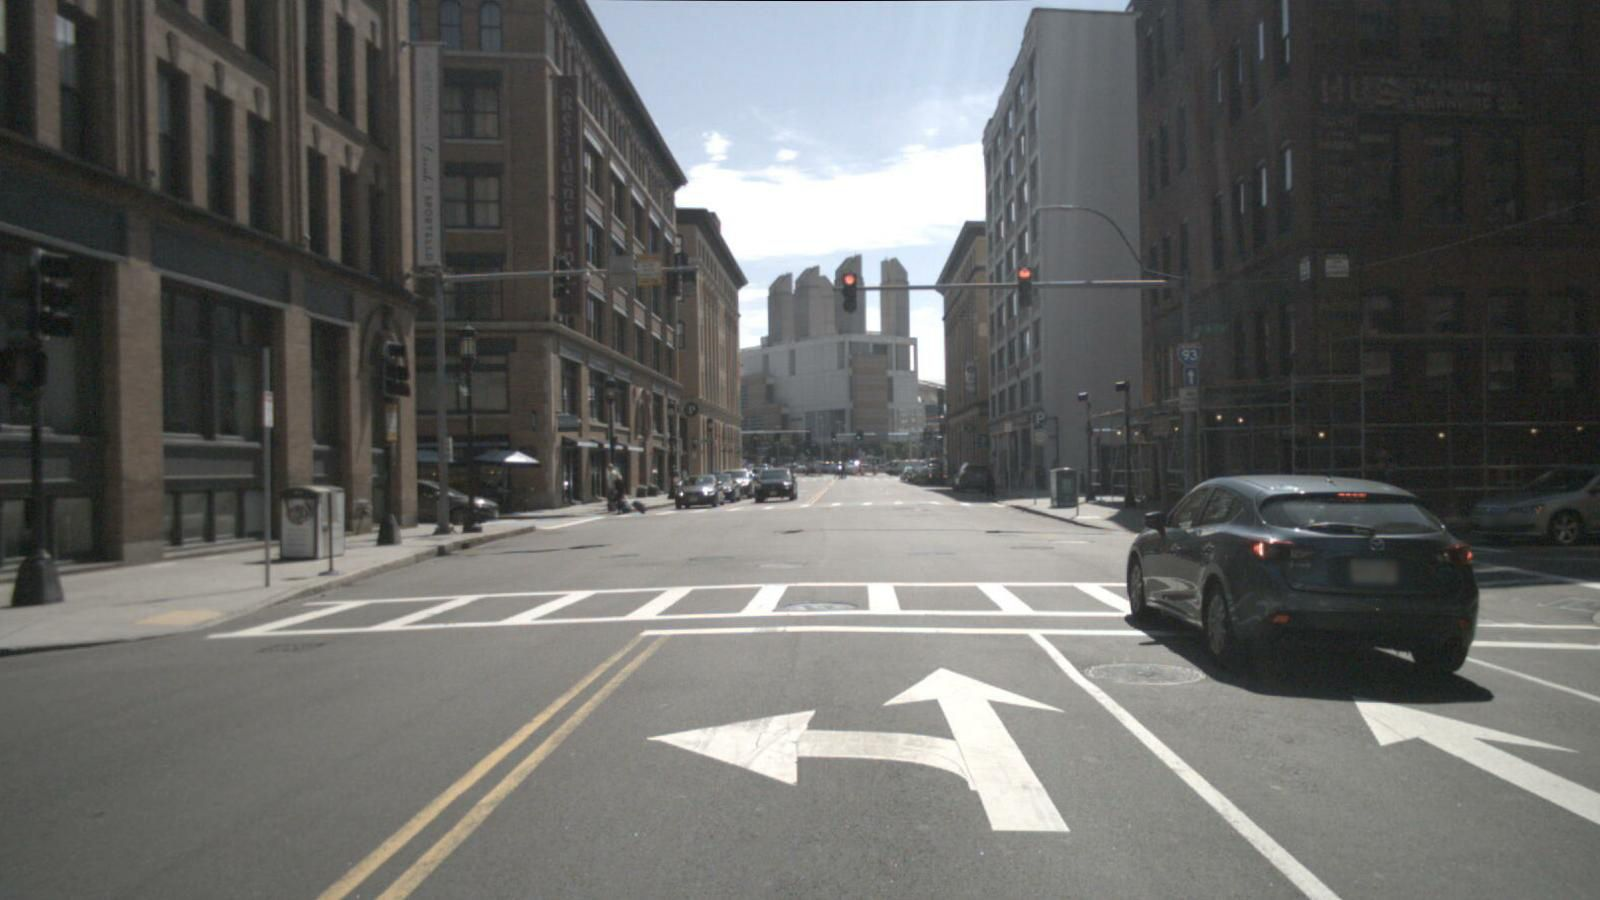
\includegraphics[width=0.3\textwidth]{Figs/depth_origin.jpg}
%              \caption{origin image}
%              \label{fig:depth_origin}
%          \end{subfigure}
         
%          \begin{subfigure}[b]{0.3\textwidth}
%              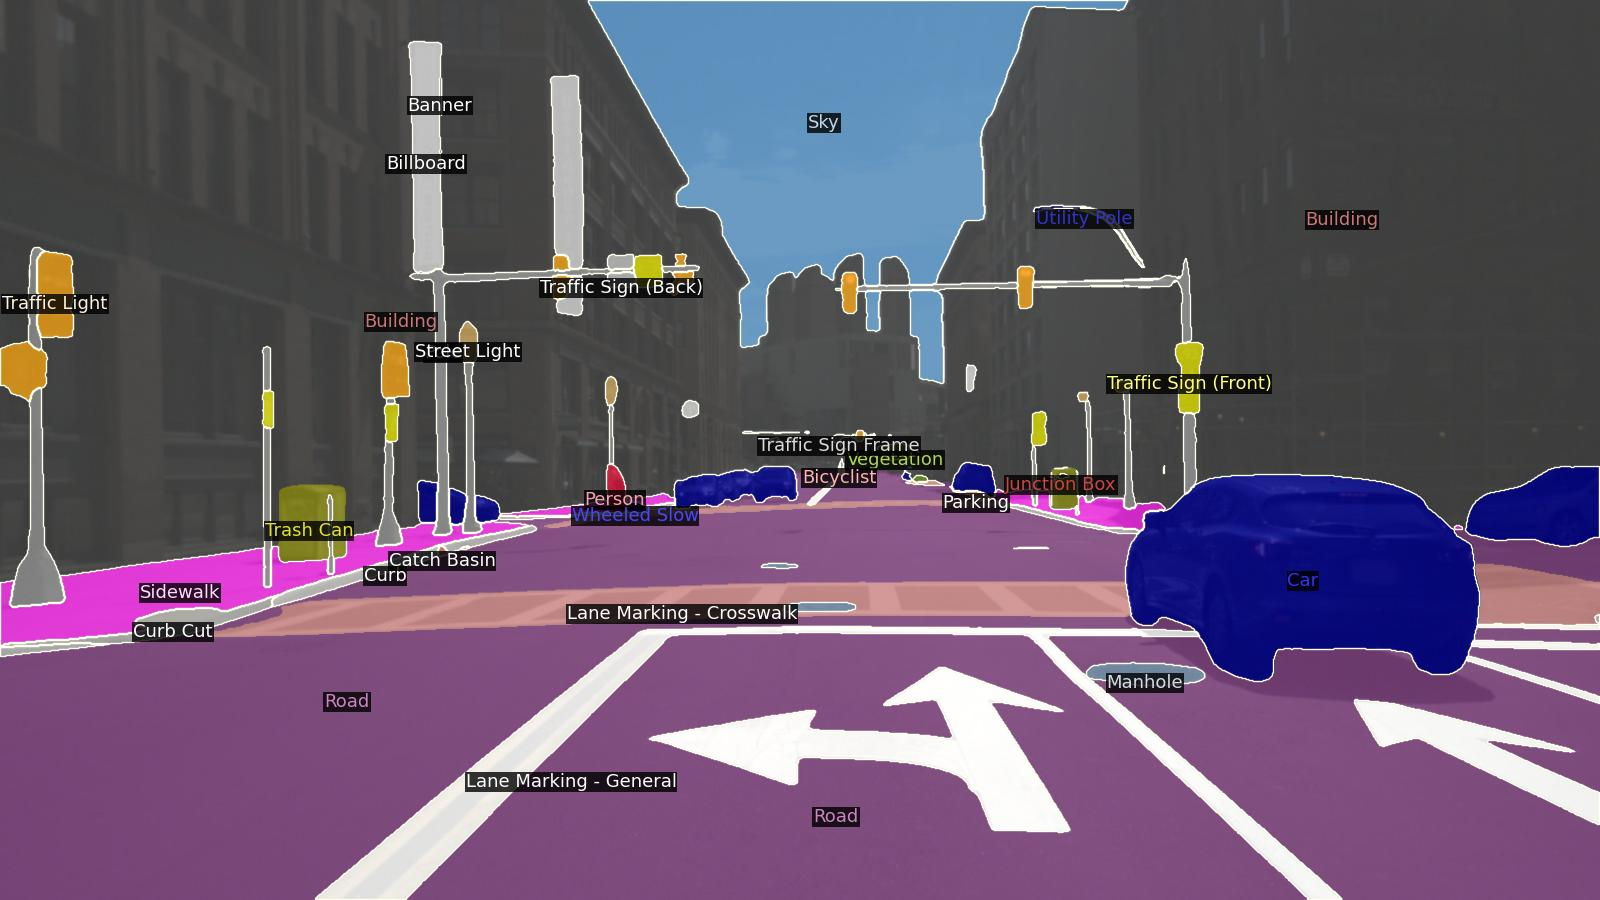
\includegraphics[width=0.3\textwidth]{Figs/depth_seg.jpg}
%              \caption{segmentation}
%              \label{fig:depth_seg}
%          \end{subfigure}
         
%          \begin{subfigure}[b]{0.3\textwidth}
%              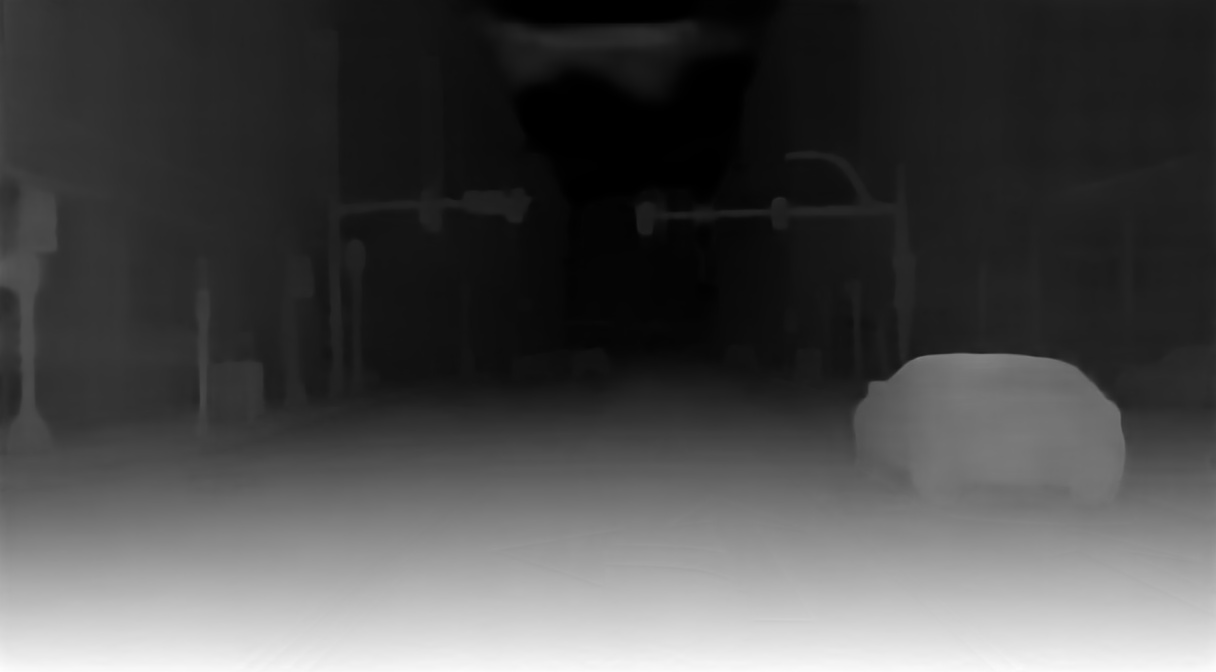
\includegraphics[width=0.3\textwidth]{Figs/depth_depth.jpg}
%              \caption{depth map}
%              \label{fig:depth_dep}
%          \end{subfigure}
%     \caption{visualization}
%     \label{fig:depth_vis}
% \end{figure}

\begin{table}[]
\centering
\caption{深度图评估 (Depth map evaluation). ARE：绝对相对误差 (absolute relative error)；SRE：平方相对误差 (square relative error)；RMSE：均方根误差 (root mean square error)；RMSE log：均方根对数误差 (root mean square logarithmic error)；$\delta$：精度 (accuracy, 阈值 1.25)}
\label{tab:depth_map_eval}
\scalebox{0.8}{
\begin{tabular}{p{0.2\textwidth}|>{\centering}p{0.13\textwidth}>{\centering}p{0.13\textwidth}>{\centering}p{0.13\textwidth}>{\centering}p{0.13\textwidth}>{\centering}p{0.13\textwidth}>{\centering}p{0.13\textwidth}>{\centering\arraybackslash}p{0.13\textwidth}}
\toprule
% \rowcolor[HTML]{C0C0C0} 
视角 (View) & ARE & SQE & RMSE   & RMSE log & $\delta$  & $\delta^2$  & $\delta^3$  \\ 
\midrule
FRONT       & 0.1522  & 3.5165 & 6.8756 & 0.2252   & 0.8720 & 0.9474 & 0.9701 \\
FRONT LEFT  & 0.2516  & 2.6591 & 5.7600 & 0.3035   & 0.7290 & 0.8755 & 0.9317 \\
FRONT RIGHT & 0.3030  & 5.9052 & 6.6903 & 0.3278   & 0.7067 & 0.8651 & 0.9231 \\
BACK        & 0.2297  & 5.5757 & 7.8486 & 0.3020   & 0.8011 & 0.9159 & 0.9535 \\
BACK LEFT   & 0.2752  & 3.6375 & 5.7691 & 0.3110   & 0.6982 & 0.8673 & 0.9279 \\
BACK RIGHT  & 0.3021  & 3.9396 & 6.2027 & 0.3413   & 0.6605 & 0.8503 & 0.9279 \\ \bottomrule
\end{tabular}}
\end{table}




\section{实验 (Experiments)}
\subsection{协议 (Protocols)}
\indent\textbf{数据集 (Dataset).}
在开环 (open-loop) 和闭环 (closed-loop) 环境下评估 ST-P3。%
%
采用 nuScenes 数据集~\cite{caesar2020nuscenes} 进行开环实验，CARLA 仿真器~\cite{dosovitskiy2017carla} 用于闭环演示。

对于 nuScenes，默认取过去 $1.0s$ 上下文，预测未来 $2.0s$ 上下文，对应过去 3 帧和未来 4 帧。
%
每个批次输入模型包含 7 帧上下文，按官方划分方法将数据集分为训练集和验证集，分别包含 26124 和 5719 个样本。

%
对于 CARLA，进行闭环评估。注意仍需要先以开环方式训练模型。
%
数据收集参照~\cite{prakash2021multi}，使用 Town05 场景进行评估，其余场景用于训练。
%
%
值得指出，CARLA 的相机配置仅包含 4 个相机，因此无法覆盖自动驾驶车辆 (SDV) 周围 $360^{\circ}$ 视场。
%
将过去 $1.0s$ 上下文和当前 4 个相机图像输入模型，生成轨迹并交由仿真器执行，直至 SDV 到达目的地或超时。
% The temporal setting is same as in nuScenes, but the spatial setting is $(40m, 40m)$ around SDV with resolution $(0.20m, 0.20m)$.


\noindent\textbf{实现细节 (Implementation Details).}
采用 EfficientNet-B4~\cite{tan2019efficientnet} 作为主干网络 (backbone)，详细模型描述见补充材料。使用 Adam 优化器，恒定学习率 $2 \times 10^{-4}$。在 4 块 Tesla V100 GPU 上以混合精度训练 20 个 epoch。
%
在 nuScenes 数据集上，BEV 空间范围为 SDV 周围 $(100m, 100m)$，分辨率 $(0.50m,0.50m)$，参照~\cite{hu2021fiery} 设置以公平比较。而在 CARLA 上，范围为 SDV 周围 $(40m, 40m)$，分辨率 $(0.20m, 0.20m)$。两个数据集相邻两帧时间间隔均为 0.5$s$。


\subsection{nuScenes 开环实验结果 (Open-loop Experimental Results on nuScenes)}

本节展示 nuScenes 数据集~\cite{caesar2020nuscenes} 上更多定性结果。同时展示学习到代价体 (cost volume) 和多种语义要素合成图的可视化。
%
注意颜色越深表示代价越小，反之亦然。如图 \ref{fig:nu_plan}-\ref{fig:nu_turning} 所示，汽车占据的位置基本都有较高代价，而可行驶开阔区域代价较低。

\begin{figure}[tb!]
    \centering
    \subfigure{
    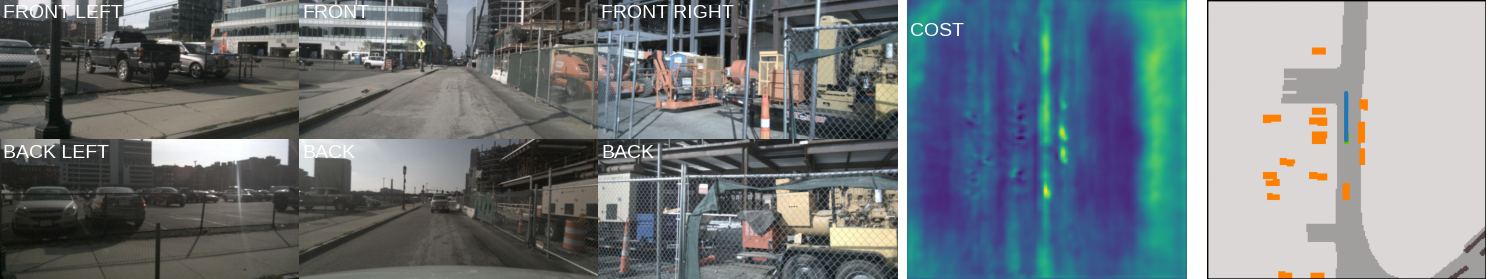
\includegraphics[width=0.98\textwidth]{Figs/nu_0319.png}
    }
    \quad
    \subfigure{
    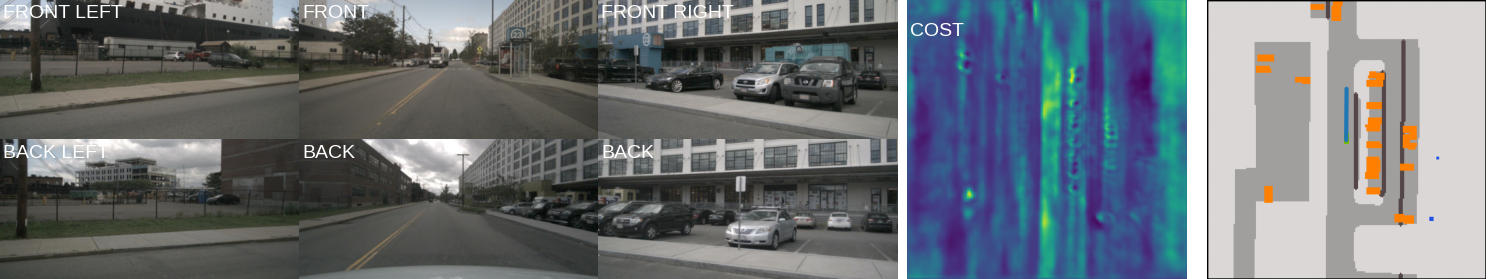
\includegraphics[width=0.98\textwidth]{Figs/nu_0169.png}
    }
    \quad
    \subfigure{
    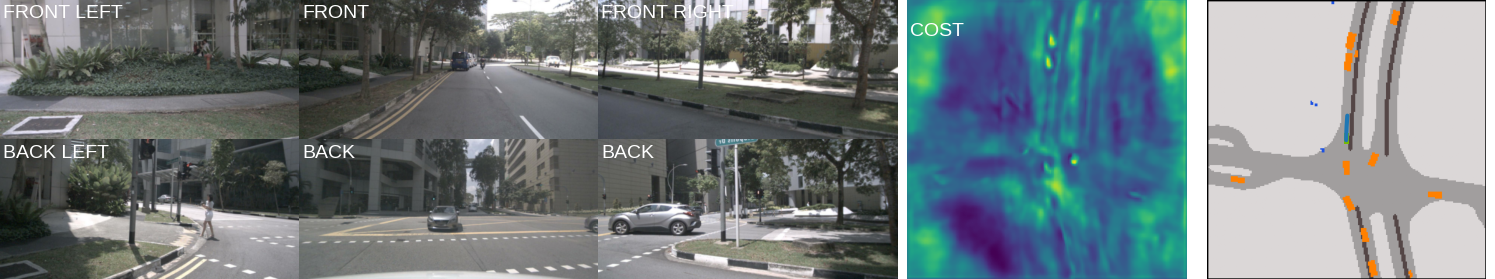
\includegraphics[width=0.98\textwidth]{Figs/nu_0295.png}
    }
    \caption{ST-P3 在直道上的定性结果 (Qualitative results of ST-P3 on the straight road)。右侧展示 BEV 中间表示和规划轨迹 (\textcolor{blue}{蓝色})，同时展示从预测模块学到子代价图。颜色越深表示代价越小}
    \label{fig:nu_plan}
\end{figure}

\begin{figure}[tb!]
    \centering
    \subfigure{
    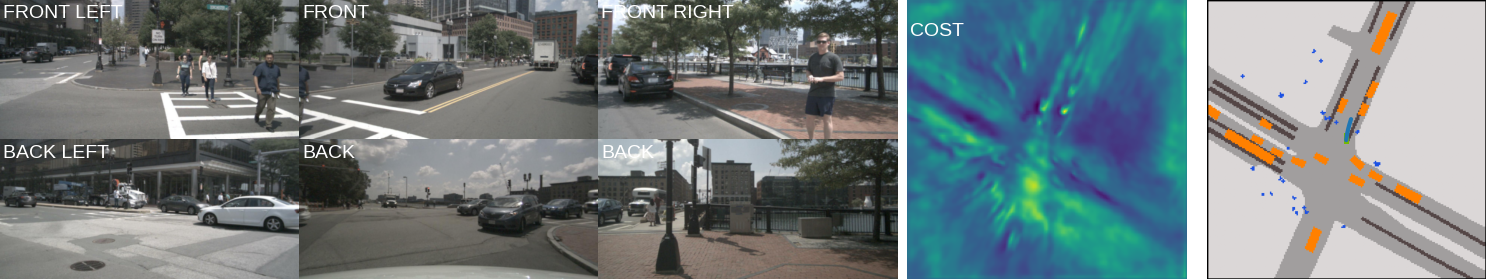
\includegraphics[width=0.98\textwidth]{Figs/nu_0021.png}
    }
    \quad
    \subfigure{
    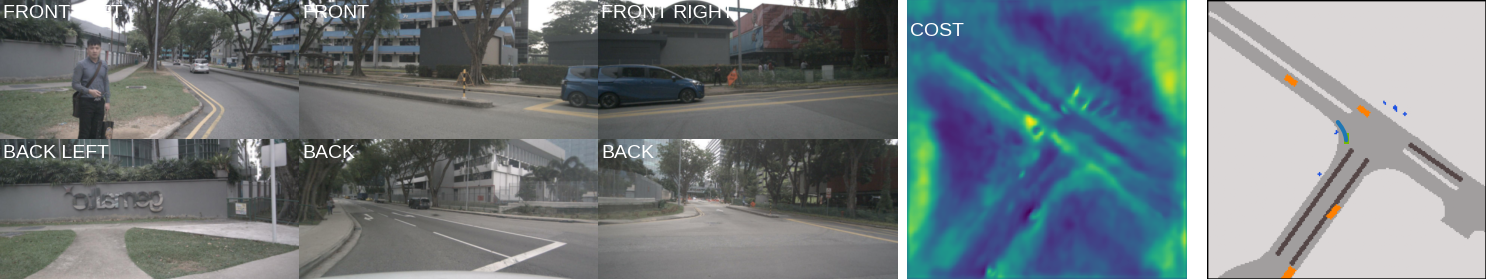
\includegraphics[width=0.98\textwidth]{Figs/nu_0044.png}
    }
    \quad
    \subfigure{
    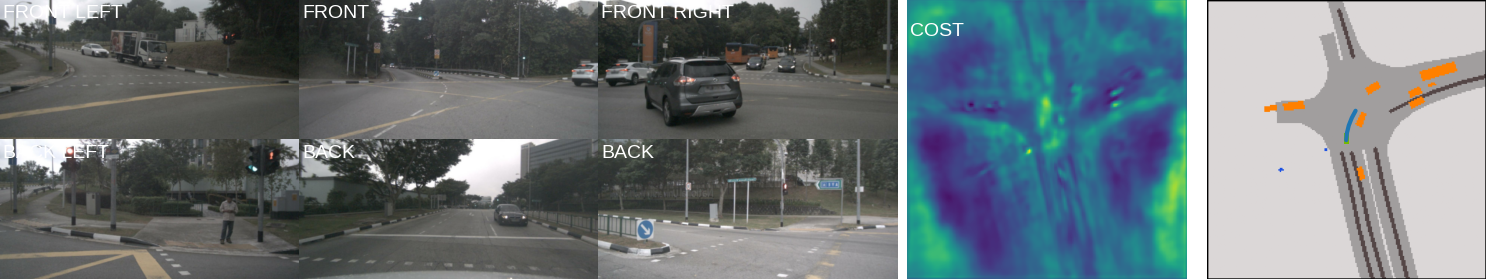
\includegraphics[width=0.98\textwidth]{Figs/nu_0376.png}
    }
    \caption{ST-P3 在交叉口转弯时的定性结果 (Qualitative results of ST-P3 when turning at intersections)}
    \label{fig:nu_turning}
\end{figure}

\subsection{CARLA 仿真器闭环规划结果 (Closed-loop Planning Results on CARLA Simulator)}
本节展示 CARLA 仿真器~\cite{dosovitskiy2017carla} 上定性结果，类似于开环结果。
%
如图 \ref{fig:error_recover} 所示，当车辆偏离车道中央时，地图检测精度显著下降。
%
这可能是由于大多数训练数据采集于正常行驶场景。
%
当地图精度较低时，使用采样器和代价图 (cost map) 的传统方法通常会偏离预期轨迹行为，但得益于优化 (refinement) 操作，车辆仍能正确行驶至预期轨迹。
%
更多不同场景可视化见图 \ref{fig:normal}-\ref{fig:turning}。

\begin{figure}[tb!]
    \centering
    \subfigure{
    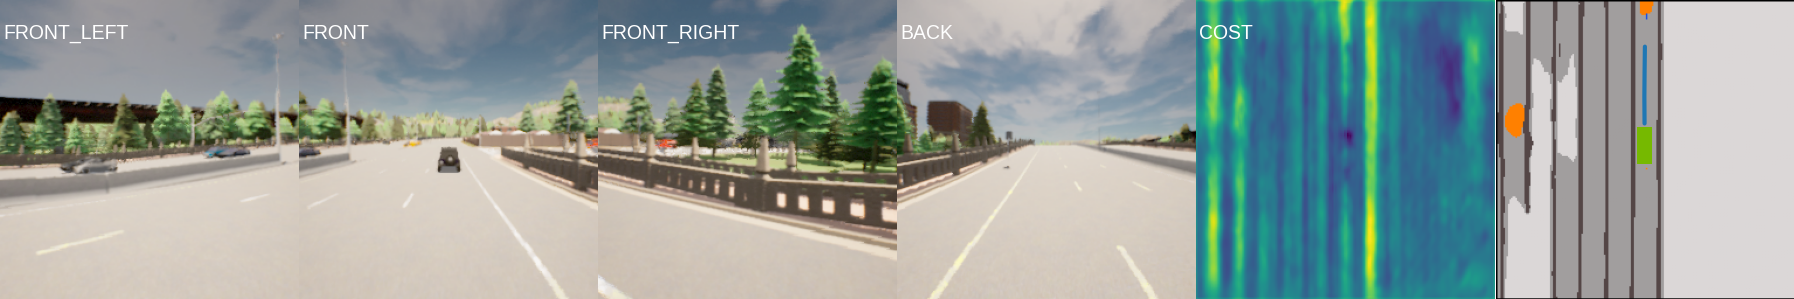
\includegraphics[width=0.98\textwidth]{Figs/0008.png}
    }
    \quad
    \subfigure{
    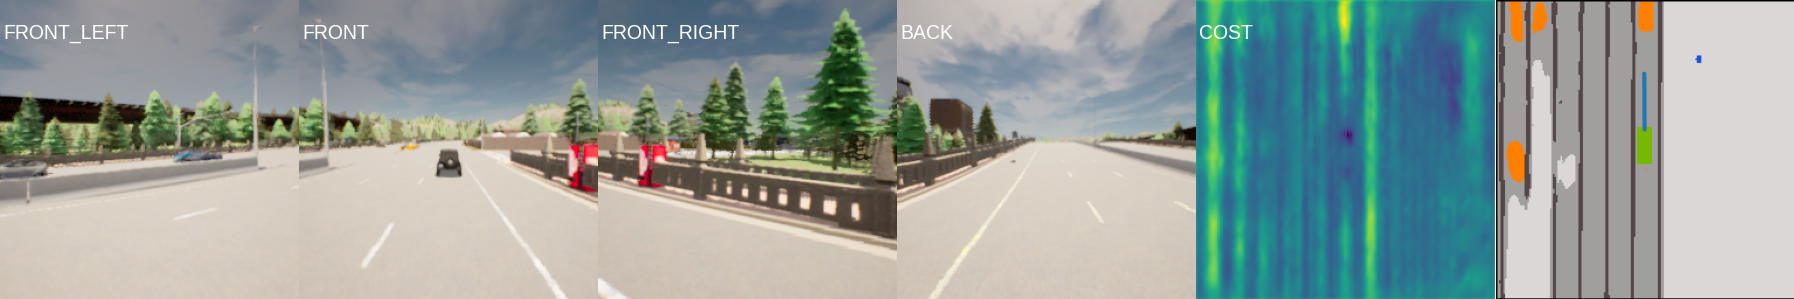
\includegraphics[width=0.98\textwidth]{Figs/0009.png}
    }
    \caption{ST-P3 在直道上的闭环规划定性结果 (Qualitative results of ST-P3 in closed-loop planning on the straight road)}
    \label{fig:normal}
\end{figure}

\begin{figure}[tb!]
    \centering
    \subfigure{
    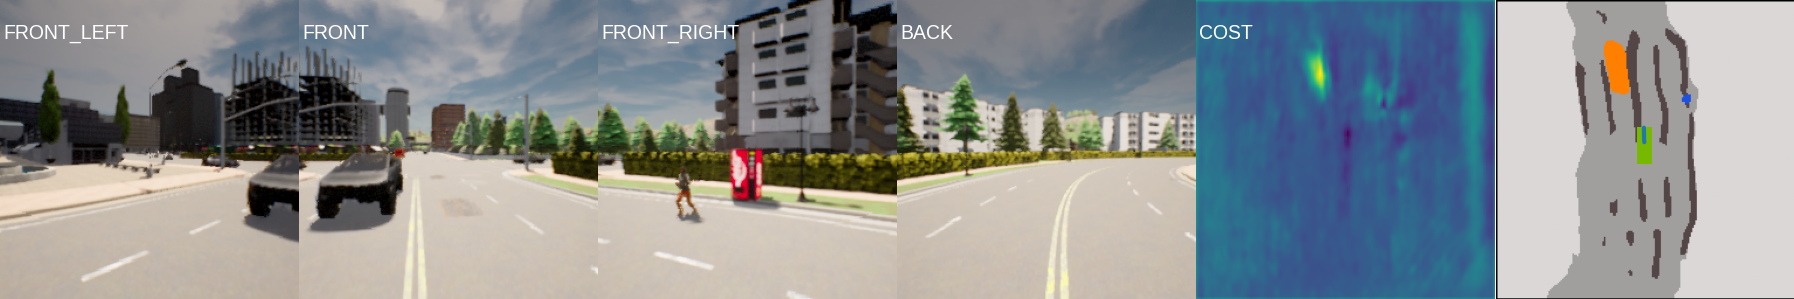
\includegraphics[width=0.98\textwidth]{Figs/0026.png}
    }
    \quad
    \subfigure{
    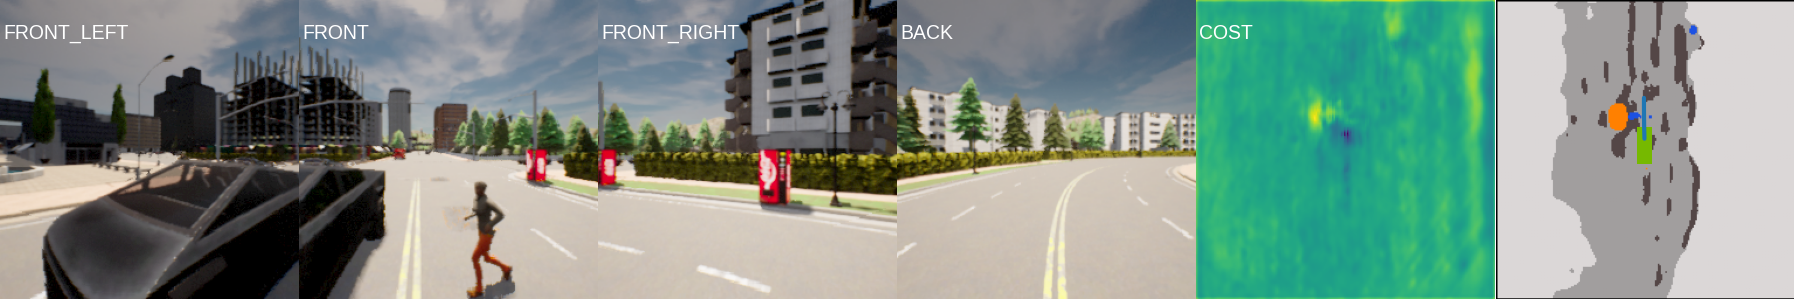
\includegraphics[width=0.98\textwidth]{Figs/0028.png}
    }
    \quad
    \subfigure{
    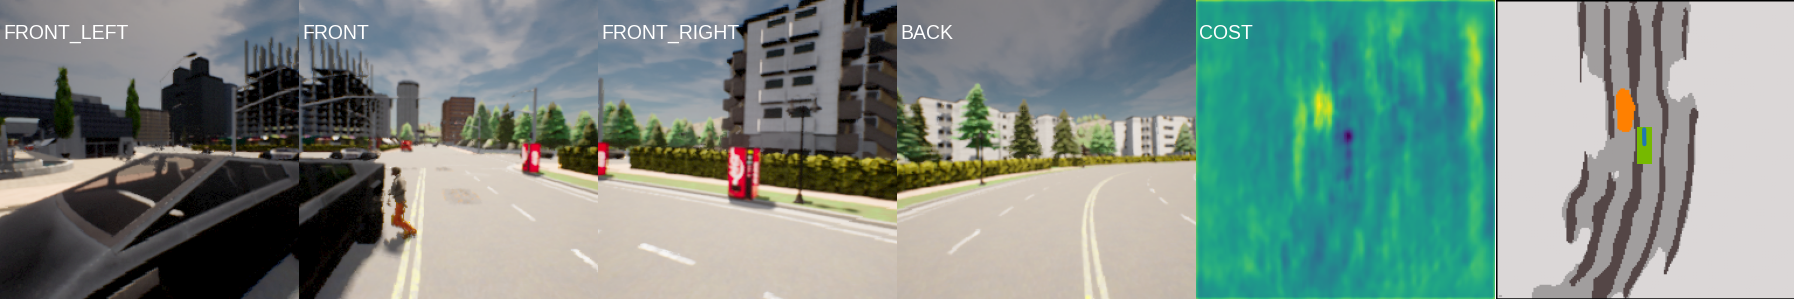
\includegraphics[width=0.98\textwidth]{Figs/0029.png}
    }
    \caption{检测到行人时 ST-P3 预测减速轨迹 (ST-P3 predicts a slowing down trajectory when detecting a pedestrian)}
    \label{fig:slow_down}
\end{figure}

\begin{figure}[tb!]
    \centering
    \subfigure{
    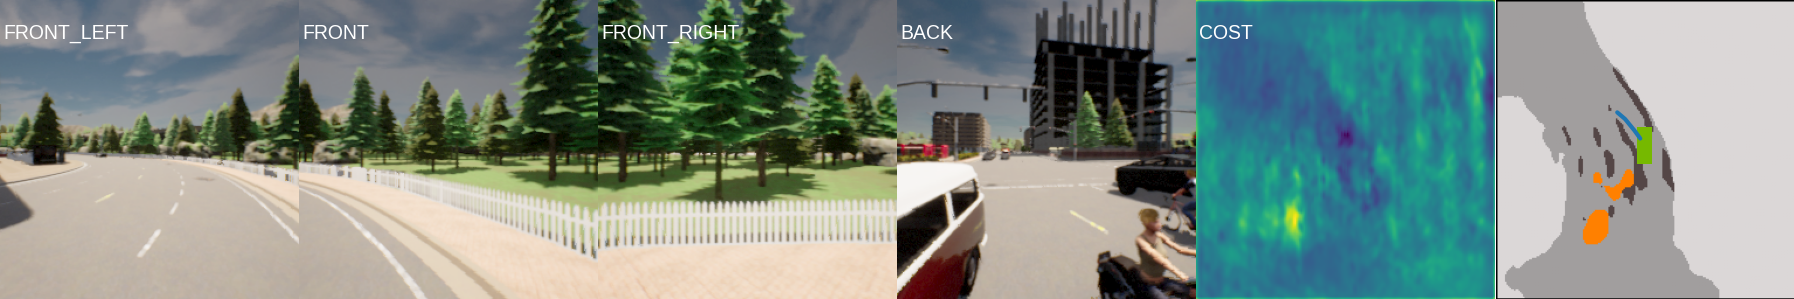
\includegraphics[width=0.98\textwidth]{Figs/0227.png}
    }
    \quad
    \subfigure{
    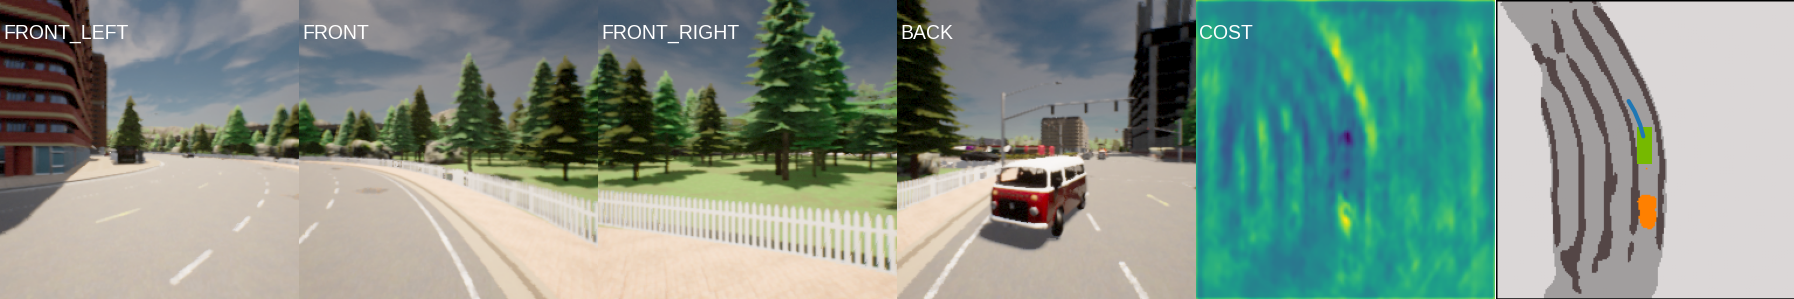
\includegraphics[width=0.98\textwidth]{Figs/0230.png}
    }
    \caption{沿预定轨迹（中心线）行驶时 ST-P3 的 BEV 表示恢复正常 (BEV representations of ST-P3 become normal when driving on a predetermined trajectory)}
    \label{fig:error_recover}
\end{figure}

\begin{figure}[tb!]
    \centering
    \subfigure{
    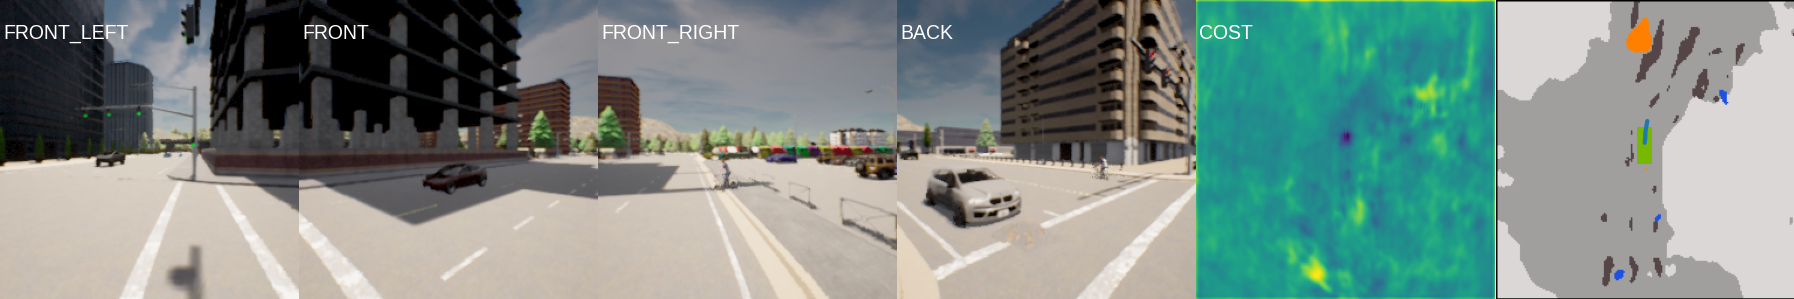
\includegraphics[width=0.98\textwidth]{Figs/0384.png}
    }
    \quad
    \subfigure{
    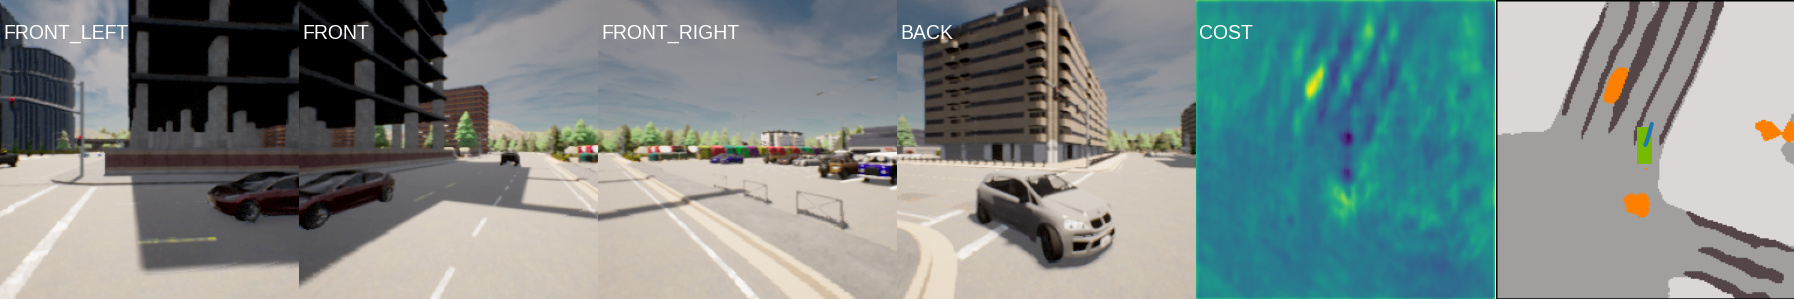
\includegraphics[width=0.98\textwidth]{Figs/0413.png}
    }
    \caption{ST-P3 在交叉口转弯时的闭环定性结果 (Qualitative results of ST-P3 in closed-loop when turning at intersections)}
    \label{fig:turning}
\end{figure}
